\documentclass[letterpaper,11pt,oneside]{article}
 
\usepackage{times}
\usepackage{epsfig}
 
\usepackage{verbatim}
 
\usepackage[none,bottom,dark,english]{draftcopy}
\draftcopyName{ DRAFT \number\day\/\number\month\/\number\year}
 
\usepackage[verbose,letterpaper]{geometry}
%\geometry{top=2cm,bottom=2cm,left=1.5cm,right=1.5cm,nohead}
\geometry{top=1in,bottom=1in,left=1in,right=1in,nohead}

\def\plotwidth{0.7\columnwidth}

\setlength{\parindent}{0pt}
\setlength{\parskip}{1.5ex plus0.5ex minus0.5ex}


\begin{document}

\title{Modelling and Shuffling}

\author{
  David R. Powell (powell@xxx), Lloyd Allison (lloyd@xxx) and Trevor I. Dix
(trevor@xxx)\\
{\small xxx=csse.monash.edu.au} \\
  School of Computer Science and Software Engineering, \\
  Monash University, \\
  Australia 3168.
}

\date{}
\maketitle

%-------------------------------------------------------------------------
\section{Introduction}
\label{sec:intro}

Most alignment algorithms assume that sequences to be aligned are random,
or perhaps that they are well described by a zero-order Markov model.
It is well known that compressible sequences,
i.e. non-random sequences of medium or low information content,
often cause false positive matches with such algorithms.
Steps to address this problem include
comparing results with those for shuffled sequences, and
masking-out sub-intervals of low information content.
Shuffling assumes a necessarily simple model of compressibility.
Masking-out is drastic because it implies that
medium or low information equals zero information which is false.
We describe a different approach to alignment which explicitly models
the statistical properties of populations of sequences and
gives the appropriate weight to each character in a sequence.
It can be used with a wide class of models of populations,
with few restrictions.
It allows models of differing complexities to be compared fairly and
it gives a natural significance test.
The method is compared to ...???...

There are many definitions of some kind
of distance, or conversely similarity, between two
sequences of values, e.g. DNA or protein sequences.
Levenshtein (1966) gave a definition of what is now known as the
(simple) edit- or evolutionary-distance where point mutations
(change, insert or delete a letter) each have a cost of one.
This metric was later studied by Sellers (1974) and many others.
Given two sequences of lengths m and n,
the well known dynamic programming algorithm (DPA), which runs in O(m*n)-time,
finds an optimal alignment that achieves the minimum edit distance.
The method can be described as cost based, simple costs (0 or 1),
global alignment.
Linear gap costs (Gotoh 1982) are more plausible in biology.
Allison (1993) showed how ad hoc weights (costs, scores) could be normalised
to reveal what probabilities for mutation steps they represent.
The local alignment problem (Sellers 1980) is to find
matching pairs of subintervals, one from each sequence.

Bishop and Thompson (1986) recognised that an alignment, optimal or not,
is just a hypothesis about how two sequences are related.
Two alignments are exclusive hypotheses so their probabilities
can be added. Allison et al (1992) extended this to
3-state models (linear gap costs) and
5-state models (piece-wise linear gap costs),
and included the model complexity,
giving a hypothesis test based on information content.

Needleman and Wunsch (1970) described an algorithm to find good matches between
two (or more) protein sequences.
To assess the significance of the match score of two sequences
they compared it to scores obtained
when "one member of the protein pair was randomized", i.e. permuted, shuffled.
Permuting a sequences preserves the zero-order statistics,
i.e. the character frequencies, but
in general destroys higher-order statistics.
Powell et al (1998) and Allison et al (1999) gave alternatives in which models
of populations of sequences are incorporated into the alignment algorithm
to weight characters appropriately.

Wrap up ...???...  our method,
local and global,
simple and linear gaps,
optimal and all alignments,
random and compressible populations. ...???...


\section{Local v. Global}

Sellers (1980) gave a precise definition for local alignment
of two sequences under the simple evolutionary (edit) distance:
"Two portions, one from each sequence, are similar if they are close
in the metric space of evolutionary distances. The method allows
a complete list to be made of all pairs of intervals,
one from each of two given sequences, such that each pair
displays a maximum local degree of similarity."

Smith Waterman ... ???...


\section{Gap Costs or Scores}

Simple point mutations rank n separated insertion (or deletion) events
the same as one event of n contiguous insertions.
It is more plausible in biology to prefer the latter over the former and
this can be modelled by linear gap costs of the form a*n+b for
constants a and b.
Gotoh (1982) gave an O(m*n)-time alignment algorithm for linear gap-costs.


\section{Optimal v. Sum over all Alignments}

Bishop and Thompson (1986) ...???...
Allison et al (1992)


\section{Random v. Compressible}

We take the terms compressible, non-random, and low information content
to be equivalent as they apply to sequences.
For example, if a DNA sequences is random, that is the probability of every
base in any context is 1/4, it is impossible to do better than to allocate
each base a fixed 2-bit code.
If something more is known about composition (zero-order statistics),
the tendency of one base to follow another (1st-order),
frequencies and run-lengths of poly-A or (AT)*, or
frequencies and similarities of ALU sequences (Herzel et al 1994), etc.,
then it is possible to predict the next base with greater than one success
in four and to design a code that is more efficient than 2-bits per base,
on average.

It is well known that low-information content sequences tend to cause
false-positive matches in alignment algorithms that assume
the data to be random, or perhaps to come from a zero-order model.
Steps to cure the problem include
significance tests that compare results against shuffled sequences, and
the masking-out of repetitive subintervals.
Needleman and Wunsch (1970)
asked "whether a particular [match score] found differs significantly
from a fortuitous match between two random sequences."
And proposed that one "construct two sets of random sequences,
from the amino acid composition of each of the proteins compared. [...]
If the [match] value found for the real proteins is significantly different
from the values found for [two of] the random sequences,
the difference is a function of the sequences alone and
not of the compositions."
We collectively call this technique and its later variations `shuffling'.

Randomly permuting a sequence preserves its zero-order statistics (composition)
but in general destroys higher-order statistics.
It is possible to shuffle a sequence while preserving its first-order
statistics and its codon usage (Fitch 1983, Altschul and Erickson 1985) but
it is hard to see how to do this while preserving its statistics under
an arbitrary model.
Even when it applies,
shuffling is only a significance test which is only half of an answer.
One or more alignments are obtained and are then tested for significance;
the significance test can only rule an alignment out.
It may be that a truly significant alignment was given a low rank,
and was ignored, by the alignment algorithm because it was
ignorant of any population model.
Shuffling cannot bring this false negative back into consideration.

...???... changing rank-order of alignments


\section{Description 1}

\begin{verbatim}
m[0,0] = z

m[i,0] = f(m[i-1,0],
           c(a[i],noCh)), i=1..|a|

m[0,j] = f(m[0,j-1],
           c(noCh,b[j])), j=1..|b|

m[i,j] = g(f(m[i-1,j-1],c(a[i],b[j])),
           f(m[i-1,j  ],c(a[i],noCh)),
           f(m[i,  j-1],c(noCh,b[j]))),
             i=1..|a|, j=1..|b|
\end{verbatim}

(a) Generic dynamic programming algorithm (DPA).


\begin{verbatim}
g = max
z = 0
f = +
c(x,x) = 1
c(x,y) = 0, x<>y
c(x,noCh) = c(noCh,y) = 0
\end{verbatim}

(b) Longest common subsequence (LCS).


\begin{verbatim}
g = max
z = 0
f = +
c(x,x), c(x,y), c(x,noCh) &
c(noCh,y) scores of choice
\end{verbatim}

(c) Arbitrary scores.


\begin{verbatim}
g = min
z = 0
f = +
c(x,x) = 0
c(x,y) = 1, x<>y
c(x,noCh) = c(noCh,y) = 1
\end{verbatim}

(d) Edit distance (0 or 1).


\begin{verbatim}
g = max
z = 1
f = *
c(x,x) = Pr(match)*Pr(x)
c(x,y) = Pr(mismatch)*Pr(x,y | x<>y)
c(x,noCh) = Pr(delete)*Pr(x)
c(noCh,y) = Pr(insert)*Pr(y)
\end{verbatim}

(e) Most probable alignment.


\begin{verbatim}
g = +
z = 1
f = *
c(x,x) = Pr(match)*Pr(x)
c(x,y) = Pr(mismatch)*Pr(x,y | x<>y)
c(x,noCh) = Pr(delete)*Pr(x)
c(noCh,y) = Pr(insert)*Pr(y)
\end{verbatim}

(f) Sum over all alignments.


\begin{verbatim}
g = logPlus where
  logPlus(-log(p1),-log(p2)) = -log(p1+p2)
z = 0
f = +
c(x,x) = -log(Pr(match))-log(Pr(x))
c(x,y) = -log(Pr(mismatch))-log(Pr(x,y|x<>y))
c(x,noCh) = -log(Pr(delete))-log(Pr(x))
c(noCh,y) = -log(Pr(insert))-log(Pr(y))
\end{verbatim}

(g) -log sum over all alignments.


\begin{verbatim}
g = max
z = 1
f = *
At m[i,j]:
 c(x,x) = Pr(match)*Pr(x|a[1..i-1],b[1..j-1])
 c(x,y) = Pr(mismatch)*Pr(x,y|x<>y,a[1..i-1],b[1..j-1])
 c(x,noCh) = Pr(delete)*Pr(x|a[1..i-1])
 c(noCh,y) = Pr(insert)*Pr(y|b[1..j-1])
\end{verbatim}

(h) Most probable alignment, non-random sequences.


1-State models, global matching.

\begin{figure}
\centering
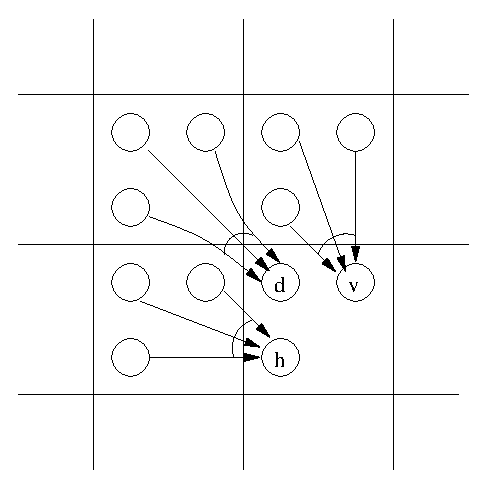
\epsfig{file=3state.eps, width=0.2\columnwidth}
\caption{\label{fig:3state}3 state mutation model aka. Affine gap costs}
\end{figure}

\begin{figure}
\centering
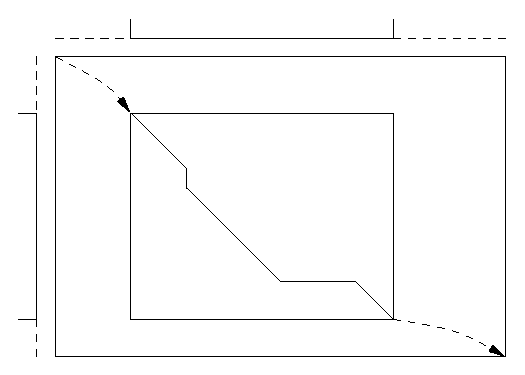
\epsfig{file=local.eps, width=0.2\columnwidth}
\caption{\label{fig:local}Local alignments}
\end{figure}


\section{Description 2}


\subsection{Adaptive sequence models}

A simple adaptive model may make the alignment algorithm behave in an
unexpected manner.  Since an adaptive model takes some time to adapt to the
sequence characters towards the start of the sequence are generally with more
bits than characters towards the end.  So, the alignment algorithm may attempt
to align characters at the start of the sequences more carefully than
characters at the end.  For this reason it is probably best to use a fitted
model instead of an adaptive model.

\subsection{Encoding of lengths}

We assume that the lengths of the two sequence being compared are encoding
independently (sensible for local alignments).  Since, we are interested only in
the difference between the null model and the alignment model and both would
encoding lengths in the same way, we may ignore them.

However, it is necessary to encode the beginning and end of the alignment in
both sequences.  Since we assume the sequence lengths have already been
encoded, and we have no other prior knowledge on where the aligned section
will be in each sequence we use a uniform prior on start and end position of
the aligned section.  Actually, we can do a little better than this.  Once the
start and end of one aligned subsequence is known and the start of other
subsequence is known, we have some knowledge about when the end of the second
subsequence will be.  This is due to the fact that the two aligned
subsequences tend to be of similar length.  So, as an approximation, we don't
encode this final position at all.  This is an underestimate, but appears to
be reasonable.  To be precise, if $l_1$ is the length of the shorter sequence
and $l_2$ the length of the longer, we encode the lengths of the un-aligned
and aligned regions in $2\log_2(l1) - 1 + \log(l2)$ bits.



\section{Tests}

-- Currently nothing about using optimal alignment.  Should there be?

Artificial data was used to compare our new alignment algorithm with the
common Smith-Waterman algorithm.  The benefit of using artificial data is that
the conditions can be controlled precisely to clearly illustrate the
advantages and disadvantages of techniques.

The implementation used for the Smith-Waterman algorithm was the \verb!prss!
program that is part of the FASTA 3.3 package.  In all tests, the \verb!prss!
program was used with the standard parameters: +5 for a match, -4 for a
mismatch, -16 and -4 for the first and subsequent characters in a sequence
respectively.  The default of 200 uniform shuffles was used to determine the
significance of each alignment.

The artificial data was generated using a number of different population
models.  In all cases, 10 parent sequences were generated from the population
model(s).  Each parent sequence was generated to be of the form $gen(50+-50)
. gen(120+-30) . gen(100+-50)$.  Where $gen(x+-y)$ mean to generate a sequence
with length selected uniform randomly from the range $[x-y, x+y]$.  Then from
each parent, 25 child sequences were generated having only the (mutated)
middle sequence in common.  Of these 25 children, 5 were generated by making
30 mutations, 5 by making 40 mutations, 5 with 50 mutations, 5 with 60
mutations and 5 with 80 mutations.  The exact method used for these mutations
is interesting in itself, but distracting at this point.  The details are
given in Appendix~\ref{sec:mutations}.  The child sequences were considered as
the library to be searched, and each parent was used in turn as the query
sequence.  Thus for each query there were 25 related sequences of differing
relatedness and 225 unrelated sequences.  This ratio of related to unrelated
sequence in the library is a high compared to real sequence databases but will
suffice for testing purposes.  Each parent sequence was compared against every
child sequence making 2500 pair-wise comparisons.  Of these 2500 comparisons,
250 are between related sequences, and 2250 between unrelated sequences.

To present the results of the tests, ROC (\cite{gribskov96, brenner98}) plots
will be used.  Each algorithm tested produces a number measuring the
relatedness of the two sequences being compared.  This may be the raw
Smith-Waterman score, or the p-value found by the \verb!prss! program, or the
log odds ratio produce by our new algorithm.  For each test, the 2500
pair-wise comparisons are ranked in order of significance by this measure.
For each possible cut-off measure the number of true positives and the number
of false positives are counted.  Plotted on the y-axis is the ratio of false
positives to the total number of unrelated pair-wise comparison.  And on the
x-axis the ratio of true positives to the total number of related comparisons.
The better an algorithm is at separating related from unrelated sequences the
closer its curve will be to the bottom right corner of the ROC plots.  Since
we are mostly interested in the behaviour for a smallish number of false
positives the y-axis is plotted with a log scale.

In the first test, the population model is the simplest possible, a uniform
model.  That is, each character occurs with a probability of 1/4.  The ROC in
Figure~\ref{fig:roc_uni} show that \verb!prss! program, the raw Smith-Waterman
score and our new algorithm perform similarly.  This test is relatively
uninteresting and is only presented to show that for high entropy sequences
our algorithms performs like existing algorithms.  Recall that our new
algorithm may take as a parameter the model for the sequences.  Except where
noted otherwise, our algorithm is told to fit a first order Markov Model to
the sequences.


\begin{figure}
\centering
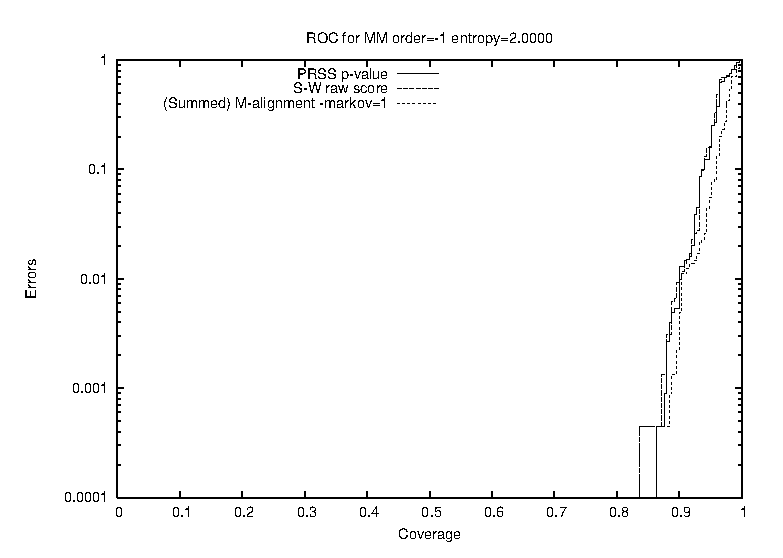
\epsfig{file=roc_uni.eps, width=\plotwidth}
\caption{\label{fig:roc_uni}ROC for a uniform sequence model.}
\end{figure}


The next test is for sequence with a biased composition, that is, sequence
from a 0th order Markov Model.  The model chosen has an entropy of 1.76 bits
per character.  The shuffling method of the \verb!prss! algorithm is designed
to account for this type of alphabet bias, and indeed, as seen in
Figure~\ref{fig:roc_0} the performance of the \verb!prss! program and our
algorithm is similar.  Also, as expected, the raw score from the
Smith-Waterman algorithm does not do a very good job at separating the related
from unrelated sequences in this case.  Since the alphabet is essentially less
that 4 here, all algorithms have more difficulty in detecting relatedness than
in the previous test.

\begin{figure}
\centering
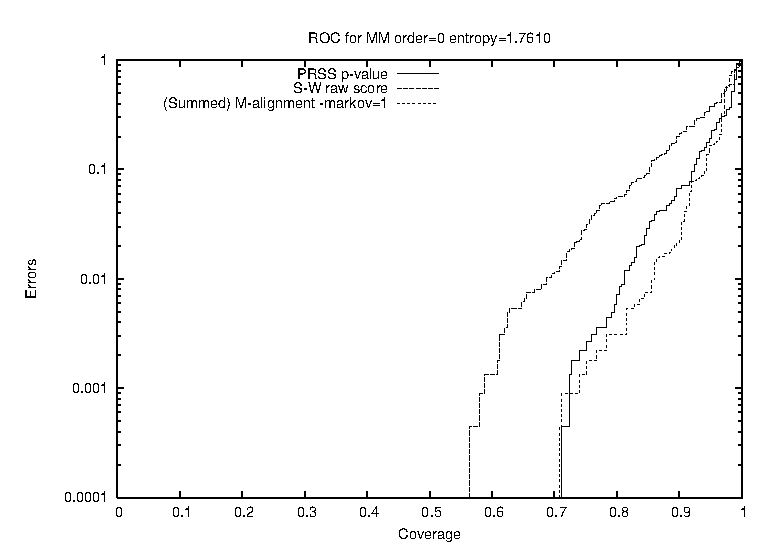
\epsfig{file=roc_0.eps, width=\plotwidth}
\caption{\label{fig:roc_0}ROC for biased composition sequences.}
\end{figure}


Figure~\ref{fig:roc_uni_0} shows the results for the next test.  In a sense,
this test is a combination of the previous two.  Instead of all 10 parent
sequences coming from the same population model, 5 come from a uniform model
(like the first test), and 5 from a 0th order Markov Model (like the second
test).  The shuffling of the \verb!prss! program does account for sequences
with a biased composition, but as seen in this test it does not perform as
well as our new method when there are different models in the population.
Similar behaviour has been seen when using a other combinations of models.

It may be argued that in practice the \verb!prss! program wouldn't use
shuffling, but would use the results of all the database searches to fit the
extreme value distribution.  NOT SURE WHAT AFFECT IT WOULD HAVE ON THIS
TEST???

\begin{figure}
\centering
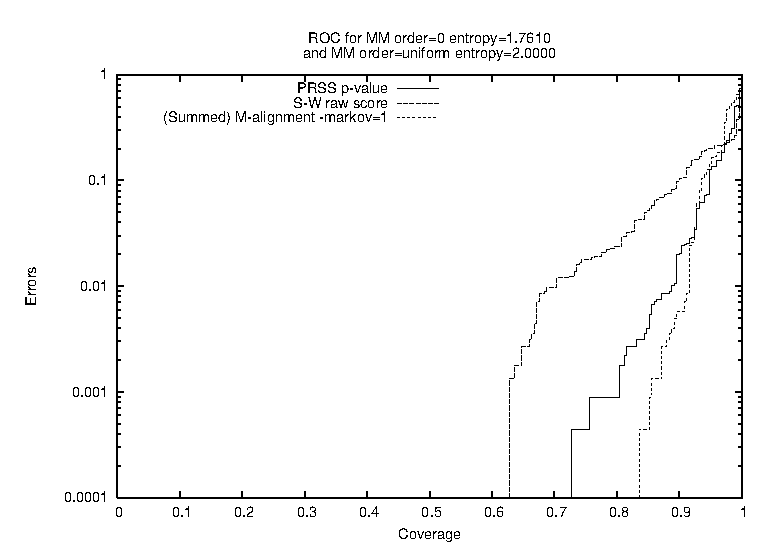
\epsfig{file=roc_uni_0.eps, width=\plotwidth}
\caption{\label{fig:roc_uni_0}ROC for a uniform sequence model and biased composition sequences.}
\end{figure}

The final test illustrates the benefits if one is able to better model the
population.  The population model in this test is a little more complicated.
This model consists of two sub-models.  One is a simple uniform model, and the
other a very biased 1st order Markov Model that produces sequences of
characters that are not unlike TATA boxes in DNA.  Sequences are generated by
choosing one of these two sub-models at random using that sub-model to produce
a random number of characters.  This is repeated a number of times to produce
a sequence of sufficient length.  This model is, in a sense, a blend between a
uniform model, with an entropy of 2 bits per character, and a 1st order model,
with an entropy of 1.1 bits per character.  Figure~\ref{fig:roc_blend} shows
the results of the different algorithms on sequences of this type.  Our
algorithm is performing significantly better than the \verb!prss! program.
The best performer in this figure is our algorithm using the ``blendModel''.
This blendModel was designed with some knowledge of the population model.
Specifically, the blendModel knows that the data is produced by a combination
of a uniform model and also the exact 1st order model used.  It does not know
the probability with which these sub-models are chosen, nor the length of the
sequence produced by the sub-models.  As can be seen in the figure, having
this extra knowledge about the population model allows for better separation
of related and unrelated sequences.  Our new algorithm is superior to the
Smith-Waterman algorithms because an arbitrary left-to-right sequence model
can be used.  Thus, more complex population models may be used with our
algorithm to allow better differentiation between related and unrelated
sequences.


It may be argued that this test is unfair to the \verb!prss! program since it
would be common practice to mask out low-complexity regions before doing the
comparison with the \verb!prss! program.  PERHAPS I OUGHT TO TEST THIS, JUST
FOR THIS CASE?

INTERESTING THAT WE DO \emph{SO} WELL IN THIS ONE COMPARED TO PREVIOUS TESTS???

\begin{figure}
\centering
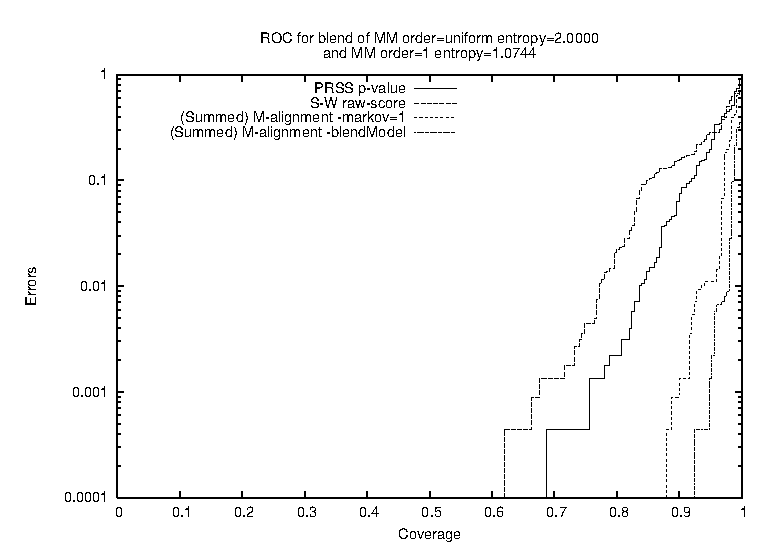
\epsfig{file=roc_blend.eps, width=\plotwidth}
\caption{\label{fig:roc_blend}ROC for a blended model}
\end{figure}


One of the advantages of our algorithm is the natural cut-off value at a
log-odds ratio of zero.  The \verb!prss! program does not have such a natural
cut-off and indeed the best value changes depending on the population of
sequences.  This may explain why our algorithm performs better in
Figure~\ref{fig:roc_uni_0}.  The tables below summarise the performance of the
algorithms for a fixed cut-off over the same data as the previous four tests.
The cut-off used for our algorithm was 0, and for the \verb!prss! program
$p=10^{-5}$ was used as this seemed to do best over all.

\begin{minipage}{\textwidth}
\small
\begin{tabular}{|l|c||c|c||c|c|} \hline
Test set & Algorithm & correct positives & incorrect positives & total related & total unrelated \\ \hline
Uni &  prss & 195 & 0 & 250 & 2250 \\ 
Uni & Sum & 226 & 14 & 250 & 2250 \\ \hline

0-order & prss & 89 & 0 & 250 & 2250 \\ 
0-order & Sum & 211 & 17 & 250 & 2250 \\ \hline

Uni \& 0-order & prss & 160 & 0 & 250 & 2250 \\ 
Uni \& 0-order & Sum & 222 & 9 & 250 & 2250 \\  \hline

Blend Uni \& 1-order & prss & 224 & 135 & 250 & 2250 \\ 
Blend Uni \& 1-order & Sum & 248 & 957\footnote{Ack! This stinks!} & 250 & 2250 \\ 
Blend Uni \& 1-order & Sum (blendModel) & 246 & 116 & 250 & 2250 \\ 
\hline \end{tabular}
\end{minipage}

\section{Conclusion}
\label{sec:conc}

\section{MAKE SURE WE HAVE THESE REFERENCED} 
normalisation.\cite{allison93a}

optimal alignment, compressible seqs.\cite{allison99}

compress 1 seq for patterns \cite{allison00a}

random seqs, sum all alignments, 1-, 3-, 5-state. \cite{allison92a}

-- shuffling+ \cite{altschul85}

-- linear gaps. \cite{altschul86}

-- Extreme value stats for alignments \cite{karlin90}

-- Blast+. \cite{altschul97}

-- simple costs, all alignments, no model complexity. \cite{bishop86}

-- shuffling. \cite{fitch83}

-- linear gap costs. \cite{gotoh82}

\cite{grumbach94}

-- ALU's form several percent of genome.\cite{herzel94}

-- original alignment paper.\cite{levenshtein66}

\cite{loewenstern97}

-- early biol, and shuffling. \cite{needleman70}

-- FASTA. \cite{pearson88}

\cite{powell98b}

\cite{rivals97}

-- edit distance. \cite{sellers74}

-- edit distance, local and global. \cite{sellers80}

-- Smith-Waterman algorithm \cite{smith81}

-- compress 1 seq for patterns. \cite{stern01}

%\bibliographystyle{abbrv}
\bibliographystyle{alpha}
\bibliography{biblio}


\appendix
\section{Mutation Model}
\label{sec:mutations}

When using a population model for sequences the problem arises of how to
mutate a sequence from this model such that the mutated sequence still
``fits'' the population model.  If characters are inserted, deleted or changed
without regard to the population model, the resulting mutated sequence will
tend towards a uniform population model.

We have a sequence, $A$, and a population model $M$.  The entropy of $A$ under
this model shall be written $M(A)$.  The length of sequence $A$ will be
written $|A|$.  The sequence that results from making $x$ mutations to $A$
shall be referred to as $A_x$.  We earlier described the motivation as wanting
the mutated sequence to ``fit'' the population model.  To make this precise,
what is desired is that as $x$ tends to infinity, the entropy of the mutated
sequence, $M(A_x)$, will tend to the entropy of the population model itself.

The method used to mutate sequences was inspired by the Metropolis
algorithm~\cite{metropolis53}.  Consider every possible sequence as having a
node, $S_i$ in a graph.  An arc between two nodes, $S_i$ and $S_j$, implies
that a single mutation relates the two corresponding sequences.  As we make
mutations to a sequence, this corresponds to moving between nodes in the
graph.  In the extreme case where many mutations are made, we want to visit
each node with a frequency equal to probability $p$, where $p$ is probability
of that node's sequence under the population model.  A sufficient condition
for this is to have the probability of taking the arc from $S_i$ to $S_j$
equal to the probability of taking the arc from $S_j$ to $S_i$.

We will assume a point mutation model for simplicity.  That is, we consider
making mutations of the form: delete a character, insert a character or change
a character.  For an alphabet of 4 characters, sequence $A$ has $3\times|A|$
possible change mutations, $|A|$ possible delete mutations and
$4\times(|A|+1)$ possible insert mutations.  If we assume a uniform, or
relatively flat, prior on the length of sequences, then we have the
requirement when mutating a sequence that on average the number of deletions
should be the same as the number of insertions.  There is a degree of freedom
in choosing the ratio of changes to insertions and deletions.  We shall use a
probability parameter $P_{change}$ for this.  We define two other probabilities
in terms of this.

$$P_{insert} = \frac{(1-P_{change})(4\times(|A|+1))}{(5\times|A|+4)}$$

$$P_{delete} = \frac{(1-P_{change})}{(5\times|A|+4)}$$

When we mutate sequence $A$, a random choice is made whether to consider an
insertion, a deletion or a change mutation using the three above probabilities
(note they sum to one).  If a deletion is to be considered, then the position
of the deletion is chosen uniform randomly over the length of the sequence.
If a change, then the position and character are chosen randomly.  If an
insertion, then the position and the character to be inserted are randomly
selected.  The sequence that would result from this mutation is $A'$.  Let
$q$ be the probability given to sequence $A$ by the population model, and $q'$
the probability given to sequence $A'$.  If $q'$ is greater than $q$ then the
mutation is accepted and $A'$ becomes $A_1$.  Otherwise, the mutation is
accepted probability $q'/q$.  This process is repeated until the desired
number of mutations has been made.

The process of calculating $q'$ from the potential mutation can be done
efficiently if the population model $M$ is such that it operates on a local
level.  That is, if $q'$ can be calculated $q$ and potential mutation in
constant time.  This is true for fixed order Markov Models.

Since this method does not preclude mutation ``undoing'' previous mutations,
the resulting mutated sequence, $A_x$, may be more similar to $A$ than
otherwise expected.  This tends to be more likely if $M$ a very low entropy
model.

In the blendModel tests we make mutations as if the population model were a
uniform model.  Thus the more a sequence is mutated the higher its entropy
will become on average.  It is possible to use the method described above to
perform population mutations correctly.  Indeed, it could done efficiently
provided information were kept about which regions of the sequence came from
which sub-model.



\end{document}
